\documentclass[12pt, letterpaper]{article}
\usepackage[utf8]{inputenc}
\usepackage{indentfirst}
\usepackage{graphicx}
\usepackage{setspace}
\usepackage[numbers]{natbib}
\usepackage [autostyle, english = american]{csquotes}
\MakeOuterQuote{"}
\usepackage{layout}
\usepackage[title]{appendix}
\usepackage[justification=centering]{caption}
\usepackage{titlesec}
\usepackage[percent]{overpic}


\begin{document}

\setcounter{secnumdepth}{-1}
\titlespacing*{\section}{0pt}{2\baselineskip}{.33333\baselineskip}

%Cover page: 5pts
%Course, subject, name, date
\title{MA348 Numerical Analysis, Thermodynamics}
\author{David Jefts}
\date{February 2, 2019}
\begin{titlepage}
	\centering
	\maketitle
	\centering
	\hfill
	\vfill
\end{titlepage}

\setlength{\voffset}{-0.5in}
\setlength{\headsep}{10pt}

%Introduction: 5pts
%Describe the problem and state objectives
\section{Introduction}
	The goal of this lab is to use various algorithms to estimate the root of a function. In this case, the function was van der Waal's equation of state, $(P+\frac{a}{v^2})(v-b)=RT$, where $P$ is the Pressure in atmospheres, $R$ is the Gas Constant for oxygen in atmospheres per mole-Kelvin, $T$ is the temperature in Kelvin, $v$ is the modal volume and $v=\frac{V}{n}$, $V$ is the total volume, $n$ is the number of moles of gas present, $a$ is the measure of the average attraction between particles, and $b$ is the volume excluded by a mole of particles. In many chemical engineering models, a very accurate modal volume of an atom or molecule, in this case oxygen,  is required in order to properly construct containment apparatuses for these gases. van der Waal's equation of state is an expansion upon the classic Ideal Gas Law formula, $PV=nRT$. Using the relationship $v=\frac{V}{n}$, the Gas Law formula used for this lab is $Pv=RT$. In this lab, the values for $R$, $a$, and $b$ are constant and known, $T$ and $P$ are not constant but known, and $v$ changes relative to the previous variables based on van der Waal's equation.

%Theory-Analysis: 5pts
%State assumptions and develop equations
\section{Theory-Analysis}
	 The function for this lab is van der Waal's equation, $(P+\frac{a}{v^2})(v-b)=RT$, and the objective is to estimate roots for this function. $v$ is the changing variable, essentially the '$x$' value, so the function must be solved in terms of $v$:

		\begin{center}
			$Pv^3-(bP+RT)v^2+av-ab=0$
		\end{center}
	
	This function serves as the main `$f(v)$' function for the remainder of this report. The Ideal Gas Law formula solved for $v$ is:

		\begin{center}
			$v=\frac{RT}{P}$
		\end{center}

	The only assumptions in this report are the oxygen Gas Constant values for $R$, $a$, and $b$. For this report, $R\approx0.082054$, $a\approx1.360$, and $b\approx0.03183$. Additionally, the Fortran installation used to compute root values is only capable of representing 16 decimal places and is ineffective at representing small numbers.

%Numerical Solution: 20pts
%Describe the numerical methods used to solve the problem
\section{Numerical Solution}
	This lab was solved using Fortran code to estimate the roots of the function and gnuplot to plot and tabulate the values. Two methods were used to compute the root values for the function- the Bisection Method and the False Position Method.

	The Bisection Method involves determining a range in which there should be a root ($[a,b]$), then finding the value at the midpoint of that range (referred to as $x_m$ and calculated with the function $\{x_m=\frac{a+b}{2}\}$). Each iteration then involves comparing $x_m$ with the function values for $f(a)$ and $f(b)$. If $\{f(a)\times f(x_m)<0\}$ then the $b$ value is replaced by $x_m$. If $\{f(a)\times f(x_m)>0\}$ then the $a$ value is replaced by $x_m$. This method iteratively moves each edge of the range closer and closer towards the true root value of the function, halving the maximum error each iteration.

	The False Position Method is very similar to the Bisection Method, except $x_m$ is calculated with the formula $\frac{[f(b)\times a]-[f(a)\times b]}{f(b)-f(a)}$. This formula is the equivalent of the secant line from $a$ to $b$, with $x_m$ the point where the secant line crosses the x-axis. In some scenarios this method can work much faster than the Bisection Method.

%Results and Discussion: 45pts
%Tabulate and plot the results, compare results, and discuss the accuracy of results
\section{Results and Discussion}
	Figure~\ref{a} is the plot of the function over the range $[0.5, 2.5]$ and shows that the solution is definitively between $2.0$ and $2.5$.

	Figure~\ref{b} in Appendix A plots the error during each iteration of the algorithm function, where each line represents one of the above-mentioned estimation methods, the x-axis is the number of iterations and the y-axis is the error. In this graph scenario $P=10atm$ and $T=300K$. This graph seems to indicate that the False Positive Roots Estimation Method both starts with a smaller error and converges towards the desired value faster. The Bisection Method converged to a solution within 52 iterations however the False Positive Method converged in 13 iterations, as shown in the table below.
	\begin{table}[]
		\centering
		\begin{tabular}{|l|l|l|}
			\hline
			n  & Bisection Error & False Positive Error \\ \hline
			1  & 2.25            & 2.090412             \\ \hline
			2  & 0.125           & 2.74E-02             \\ \hline
			3  & 6.25E-02        & 1.37E-03             \\ \hline
			4  & 3.13E-02        & 6.75E-05             \\ \hline
			5  & 1.56E-02        & 3.32E-06             \\ \hline
			6  & 7.81E-03        & 1.63E-07             \\ \hline
			7  & 3.91E-03        & 8.04E-09             \\ \hline
			8  & 1.95E-03        & 3.96E-10             \\ \hline
			9  & 9.77E-04        & 1.95E-11             \\ \hline
			10 & 4.88E-04        & 9.57E-13             \\ \hline
			11 & 2.44E-04        & 4.71E-14             \\ \hline
			12 & 1.22E-04        & 2.66E-15             \\ \hline
			13 & 6.10E-05        & 0                    \\ \hline
			14 & 3.05E-05        &                      \\ \hline
			15 & 1.53E-05        &                      \\ \hline
			16 & 7.63E-06        &                      \\ \hline
			17 & 3.81E-06        &                      \\ \hline
			18 & 1.91E-06        &                      \\ \hline
			19 & 9.54E-07        &                      \\ \hline
			20 & 4.77E-07        &                      \\ \hline
			$...$ & $...$           &   $...$          \\ \hline
			45 & 1.42E-14        &                      \\ \hline
			46 & 7.11E-15        &                      \\ \hline
			47 & 3.55E-15        &                      \\ \hline
			48 & 1.78E-15        &                      \\ \hline
			49 & 8.88E-16        &                      \\ \hline
			50 & 4.44E-16        &                      \\ \hline
			51 & 4.44E-16        &                      \\ \hline
			52 & 0               &                      \\ \hline
		\end{tabular}
		\caption{Table of values for the error on each estimation method}
		\label{err_table}
	\end{table}
	
%Conclusions: 20pts
%Comment on the efficiency of the solvers
\section{Conclusions}
	The False Positive Method appears to be much more efficient without sacrificing any error, in the future that may not always be the case though. If this were to be done by hand the most accurate way would be the False Positive Method as the Bisection Method is much slower to converge. There are other ways to optimize this function. The Bisection and False Positive Methods of finding roots are just a two from a plethora of various solvers and algorithms that accomplish the same this. 

\pagebreak
	
%Appendices
%Include listings of the source codes, include printed copies of the output files
\appendix
	\section{Appendix A}
		Important Graphs
		\begin{figure}[htp]
			\centering
			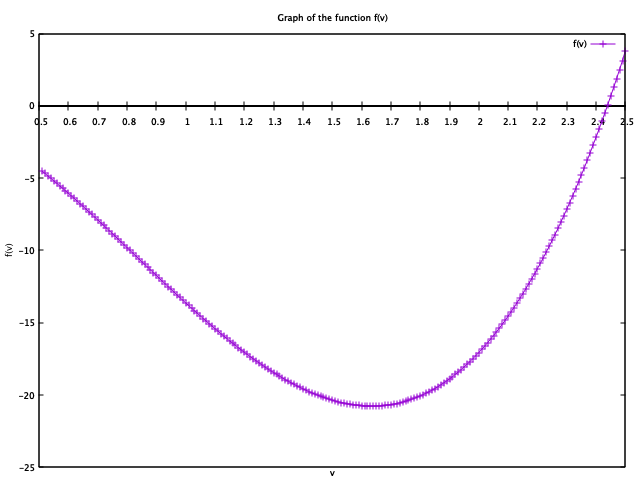
\includegraphics[width=\linewidth]{f(v)-plot.png}
			\caption{Graph of the $f(v)$ function}
			\label{a}
		\end{figure}
		\begin{figure}[htp]
			\centering
			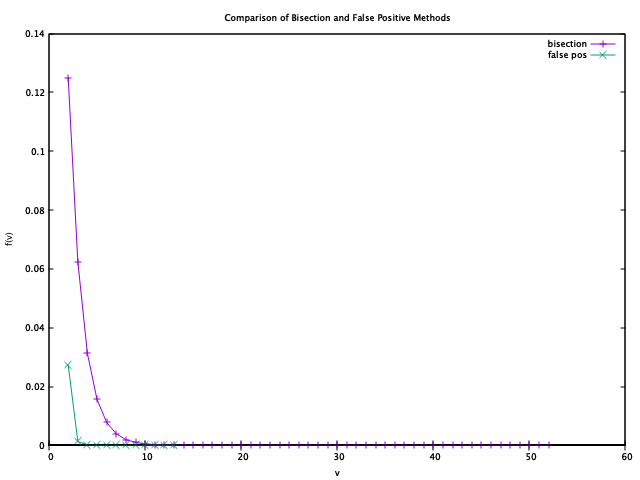
\includegraphics[width=\linewidth]{bisecVSfalse.png}
			\caption{Bisection and False Position Errors when $P=10atm$ and $T=300K$}
			\label{b}
		\end{figure}

	\pagebreak

	\section{Appendix B}
		Graphs of each combination of Pressure/Temperature. The green line represents the graph of the Ideal Gas Law on the interval while the purple line represents the False Position Estimation function on the interval. $v$ is the modal volume estimated by the False Position Method.
		
		%1 atmosphere of Pressure
		\begin{figure}[htp]
			\centering
			\begin{overpic}[width=0.5\textwidth]{1&300.png}
				\put (15,35) {\huge$\displaystyle v=24.592799$}
			\end{overpic}
			\caption{$P=1atm$, $T=300K$}
		\end{figure}

		\begin{figure}[htp]
			\centering
			\begin{overpic}[width=0.5\textwidth]{1&500.png}
				\put (15,35) {\huge$\displaystyle v=41.025704$}
			\end{overpic}
			\caption{$P=1atm$, $T=500K$}
		\end{figure}

		\begin{figure}[htp]
			\centering
			\begin{overpic}[width=0.5\textwidth]{1&700.png}
				\put (15,35) {\huge$\displaystyle v=57.445966$}
			\end{overpic}
			\caption{$P=1atm$, $T=700K$}
		\end{figure}
		
		%10 atmospheres of Pressure
		\begin{figure}[htp]
			\centering
			\begin{overpic}[width=0.5\textwidth]{10&300.png}
				\put (15,35) {\huge$\displaystyle v=2.438403$}
			\end{overpic}
			\caption{$P=10atm$, $T=300K$}
		\end{figure}

		\begin{figure}[htp]
			\centering
			\begin{overpic}[width=0.5\textwidth]{10&500.png}
				\put (15,35) {\huge$\displaystyle v=4.101629$}
			\end{overpic}
			\caption{$P=10atm$, $T=500K$}
		\end{figure}

		\begin{figure}[htp]
			\centering
			\begin{overpic}[width=0.5\textwidth]{10&700.png}
				\put (15,35) {\huge$\displaystyle v=5.752097$}
			\end{overpic}
			\caption{$P=10atm$, $T=700K$}
		\end{figure}

		%100 atmospheres of Pressure
		\begin{figure}[htp]
			\centering
			\begin{overpic}[width=0.5\textwidth]{100&300.png}
				\put (15,35) {\huge$\displaystyle v=0.226358$}
			\end{overpic}
			\caption{$P=100atm$, $T=300K$}
		\end{figure}

		\begin{figure}[htp]
			\centering
			\begin{overpic}[width=0.5\textwidth]{100&500.png}
				\put (15,35) {\huge$\displaystyle v=0.411614$}
			\end{overpic}
			\caption{$P=100atm$, $T=500K$}
		\end{figure}

		\begin{figure}[htp]
			\centering
			\begin{overpic}[width=0.5\textwidth]{100&700.png}
				\put (15,35) {\huge$\displaystyle v=0.584196$}
			\end{overpic}
			\caption{$P=100atm$, $T=700K$}
		\end{figure}

	\clearpage
	
	\section{Appendix C}
		\begin{figure}[h]
			\centering
			%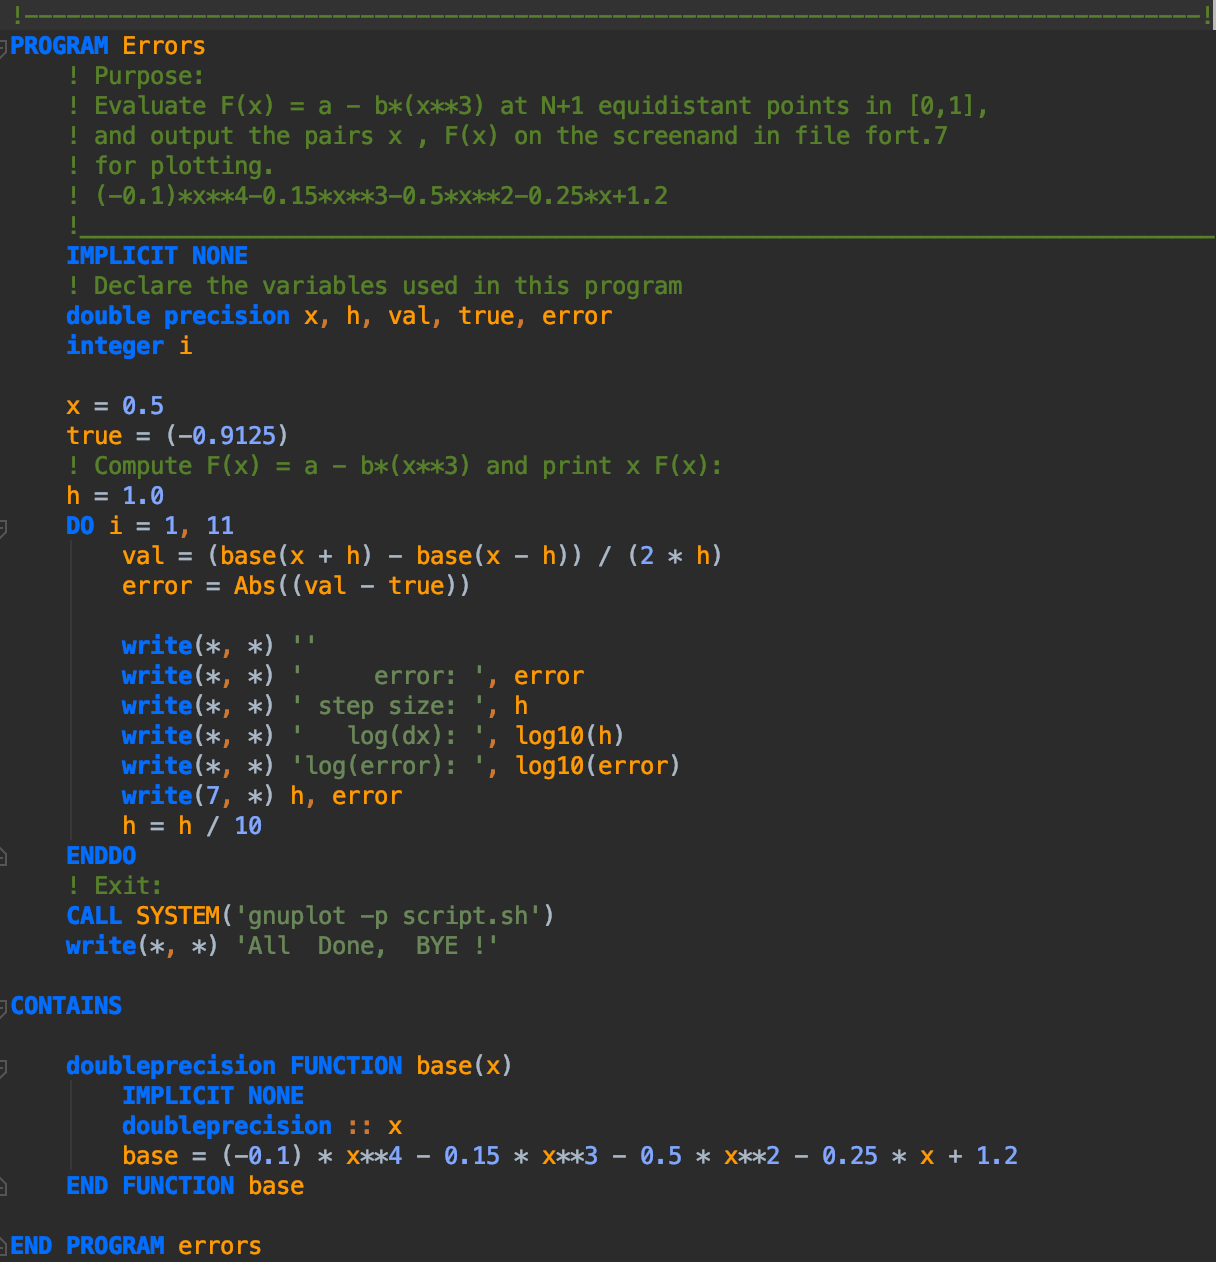
\includegraphics[width=\linewidth]{FortranCode.png}
			%\caption{Fortran program code}
		\end{figure}
		
		\begin{figure}[h]
			\centering
			%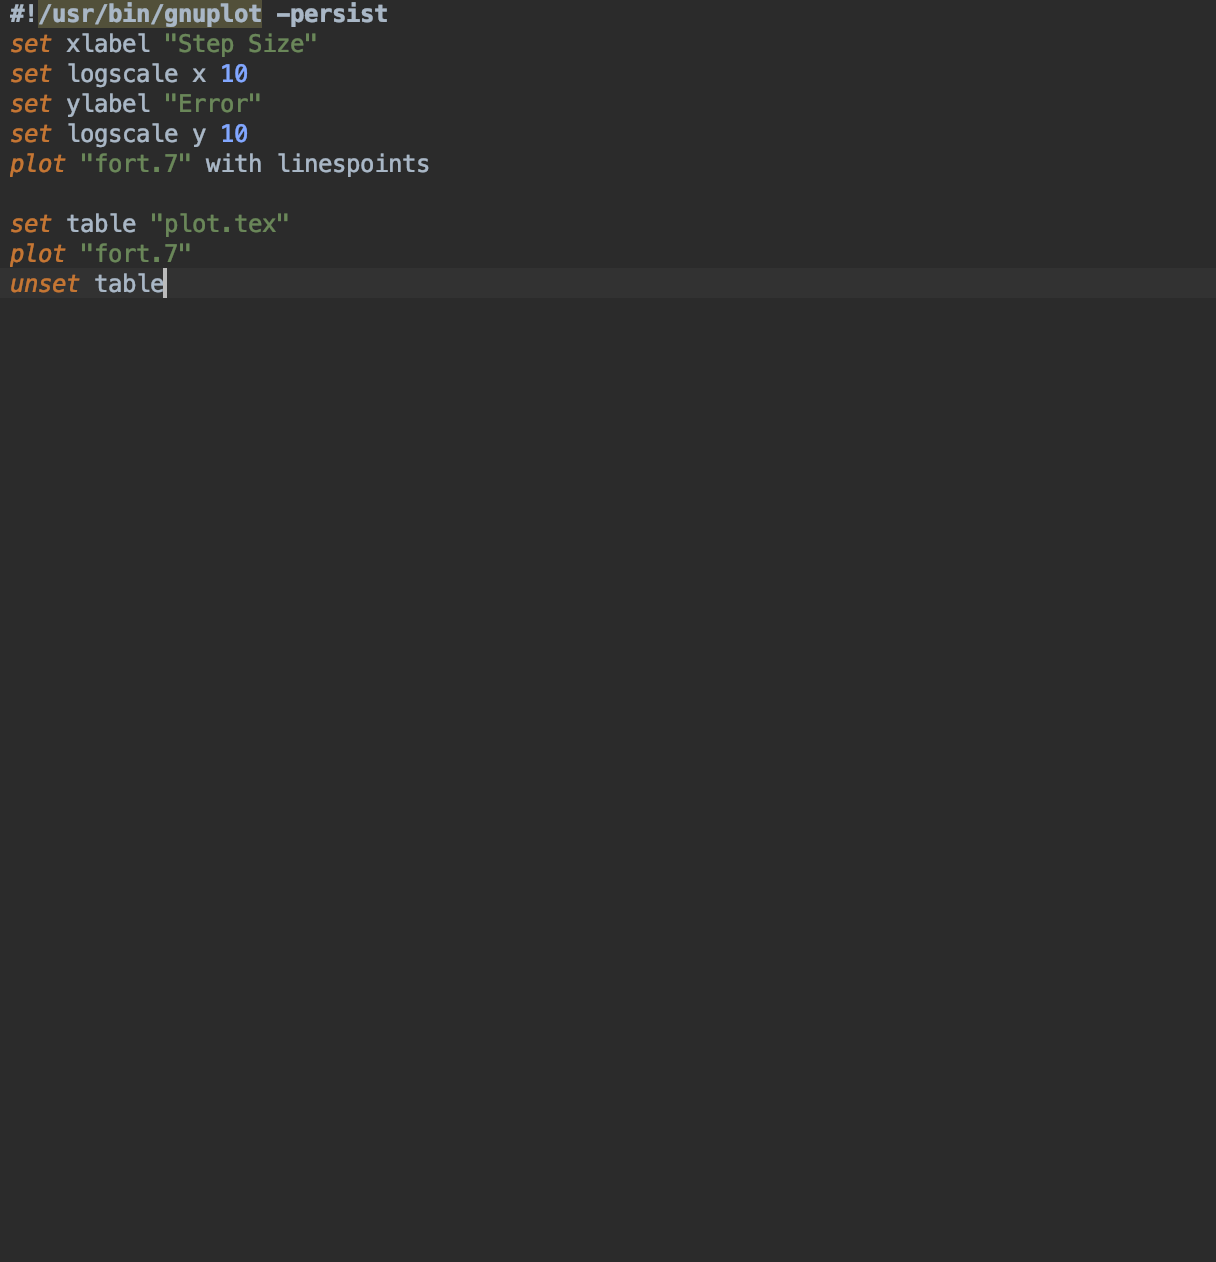
\includegraphics[width=\linewidth]{GnuplotCode.png}
			%\caption{Script for gnuplot to set up the graph correctly}
		\end{figure}


\end{document}
